\documentclass{cranfieldChart}


\begin{document}

\maketitle{Group project - G2}
{Q. Diaferia\\
T. Levasseur\\
G. Perez Bada\\
P. Wang
}{Group project}{Group 2 - MeshSlicer}{cover.png}

\newpage
\tableofcontents
\newpage

\begin{abstract}
The traditional way to write software application is serial, and instructions are executed on a single processor one after another.
As scientific simulation problem's size grows, this way becomes more and more time consuming and is no longer suitable. This is why we introduce the notion of parallel computing: the simultaneous use of multiple processors to solve a single and large size computational problem. One of the important approach to parallel computing is the distribution of memory and problem partitioning. Partitioning a problem can be challenging since the total work load should be divided in a way that processors share the same amount of work load and inter-processor communication time is minimized. In order to simplify the graph problem and so make the partitioning problem easier, we introduce another phase before computing the partition phase: coarsening phase, where a matching of edges is performed and vertices incident on these edges are collapsed together. We also introduce a final phase: refinement phase which reform the partitioned graph to it original form. Our work aims to address the challenge of partitioning graphs using an open source library: METIS. We conducted a website that enables users to connect to Astral resources remotely and partition their graphs online in a timely fashion. 
\end{abstract}
\newpage
\section{Market Analysis}
Graph partitioning could be useful to a great range of industries as well as research laboratories. Its several important applications lay on VLSI circuit layout, image processing, solving sparse, linear systems and distributing workloads for parallel computing. Our initial aimed customers are industries that boast super computer equipments.
\section{Feasibility Analysis} 
\paragraph{}
Before specifying the requirements of this project, we first study its feasibility. That is, technical feasibility, economical feasibility and organisation feasibility. We first tested if the two applications that we would be using to partition graphs were working properly. Then, we made sure that our website prototype could connect users with their Astral ID and password remotely to Astral. Since the two partition applications are free, we are able to run this project without any financial restraint. We paid a visit to the Cranfield IT department to required whether it was possible for an external company to reach an agreement with Cranfield University to obtain extra Astral ID. The answer was no. So we fixed our target customers as those who already had Astral accounts. The only risk would lay on network connection. 

\section{High level description of our website}
\paragraph{}
This is a website application that enable user who hold a valid Cranfield Astral ID and password to upload graphs, select a partition method, choose an initial partition scheme, a refinement scheme, the number of parts in which to split the graph, set the maximum load imbalance, decide the weight of each partition and either they want to minimize edge cut or volume. 
\paragraph{}
Once the setting is finished, the partitioning will be done remotely on Astral and the results will be sent back to the web interface where our users will be able to collect the output files containing the partitioned graph as well as downloading them to their local PC. 

\section{Architecture of our system}

\begin{figure}[h]
\centering
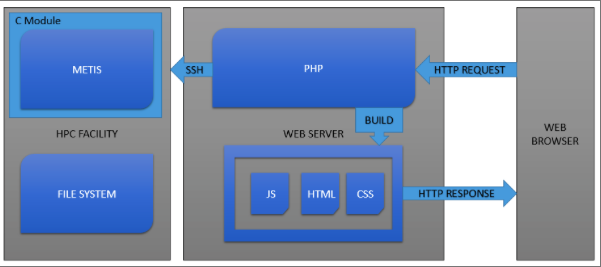
\includegraphics[width=0.8\textwidth]{ressources/architect}
\label{architect}
\caption{System architecture}
\end{figure}

\paragraph{}
In general, our application is a web-based, three-tier, client-server system. On the client side, the web browser first send a http request to the web server in which the PHP script will interpret the request and remotely connect to the HPC faculty. Once the computation is done by $Metis$ which should be installed on the HPC faculty beforehand, the PHP script will build automatically a web page that contains JavaScript, HTML and CSS code. Finally, the web page will be display on the web browser. 

\section{Requirement Analysis}
\subsection{System functional requirements specification}
This a web application that allows users to partition graphs and mesh on-line in a timely fashion. 
\begin{itemize}
    \item The application shall allow user to log in with a valid Cranfield Astral user ID and password. 
    \item Once the user is logged in, the application shall allow him to upload graphs or meshes in form of $graph_name.graph$ and $mesh_name.mesh$ from his local PC. 
    \item The application shall be able to remotely use $MeTis$ as open sources for partitioning located on Astral system. 
    \item The application shall allow the user to select a partition method between k-way and recursive bisection.
     \item The application shall let the user set either if he wants to minimize the edge cut or communication of the graph.
    \item The application shall allow the user to choose one initial partition scheme between:
        \begin{itemize}
             \item Greedy bisection
            \item Random bisection and refinement 
        \end{itemize}
    \item The application shall allow the user to choose on coarsening method between: 
        \begin{itemize}
            \item Random matching 
            \item Heavy edge cutting 
        \end{itemize}
    \item The application shall allow user to set if the partition is contiguous or not. 
    \item The application shall allow user to set the maximum load imbalance via x with $L= (1+x)/100$
    \item The application shall let the user set the number of parts in which to split the graph. 
    \item If the user choose to partition a mesh, the user shall be able to mesh type between: 
    \begin{itemize}
        \item Dual Graph
        \item Nodal Graph 
    \end{itemize}
    \item Once the user finish setting the partition preferences and click on the launch partition, a video window will pop up and he or she shall be able to view the whole partitioning process as the origin graph will be painted on different colors which represents different partition group. 
    \item The application shall allow users to download the output file to his local PC. Original output file of the $Metis$ application contains only one index number on each line which represents a node of the graph and the index number means the processor to which it has been assigned. 
    \item User shall be able to delete any file from his repository. 
    \item User shall be able to log out at any time. 
\end{itemize}
    
\subsection{System non functional requirements specification}
    \begin{itemize}
        \item Users' log in security should be verified. User's ID and password shouldn't be given out under any circumstances. 
        \item The application respond time shall be in order of second. 
        \item The application shall be easy to use without tutorial needed, but description of different partition methods and refinement schemes shall be included on the website.
     \end{itemize}
     
\section{Usage of tools}
\paragraph{}
We decided to use $Metis$, an open source software, to compute data partition. They are well known for producing high quality partitions in a timely fashion and being actively supported. 

\section{Use case diagram}

\begin{figure}[h!]
\centering
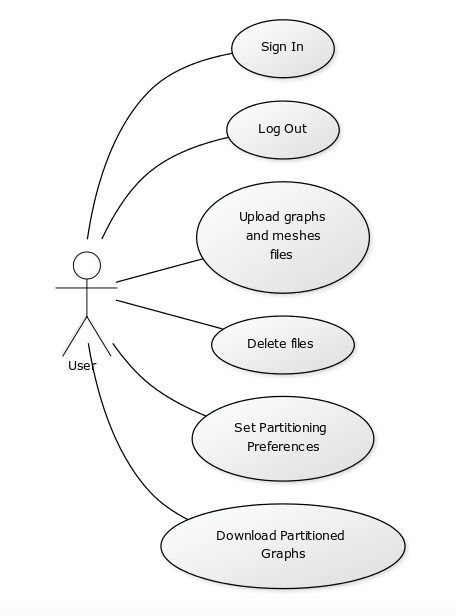
\includegraphics[width=0.8\textwidth]{ressources/use-case}
\label{use-case}
\caption{Use case diagram}
\end{figure}

\paragraph{}
We define only the user as an actor in our system as we use remotely Astral resource to control access, manage users' information and users' input and output files. In general, our web application serves as a platform to enable users to connect remotely to Astral and use its resources ($Metis$ in our case).

\paragraph{}
Definition of actions: 
\begin{itemize}
    \item Sign in 
    \item Log out
    \item Upload graphs and meshes
    \item Set Partitioning Preferences 
    \item Download Partitioned Graphs 
\end{itemize}
As described earlier, our users shall be able to set the partition preferences. The setting requirements are predefined on $Metis$ as input parameters. Our job is to provide a link between the web interface and $Metis$ so that the setting preferences will be used as configuration input to launch the partitioning on $Metis$. Setting parameters are as followed:
\begin{itemize}
    \item Graph/Mesh 
    \begin{itemize}
        \item Graph:0
        \item Mesh: 1
    \end{itemize}
    \item Partition method
    \begin{itemize}
        \item Bisection:0
        \item K-way: 1
    \end{itemize}
    \item Partition objective
    \begin{itemize}
        \item Edge cut: 0
        \item Communication volume: 1
    \end{itemize}
    \item Coarsening scheme
    \begin{itemize}
        \item Random: 0
        \item Heavy-edge : 1
    \end{itemize}
    \item  Initial partition scheme
    \begin{itemize}
        \item Greedy: 0
        \item Random bisection + refinement: 1
        \item Edge cut derived: 2
        \item Node-based greedy: 3
    \end{itemize}
    \item Contiguous partition
    \begin{itemize}
        \item No: 0
        \item Yes: 1
    \end{itemize}
    \item Imbalance value $x$
    \begin{itemize}
        \item Default: 0
        \item Integer: $x$
    \end{itemize}
    \item Number of parts 
    \item Mesh based
    \begin{itemize}
        \item Dual graph: 0
        \item Nodes: 1
    \end{itemize}
\end{itemize}

\section{How we manage the project and tasks partition}
\paragraph{}
After our first meeting, we first analysed the total work load of the project and established a to-do list. We exchanged each group member's strengths and divided tasks accordingly. We used $Trello$ and $GitHub$ as real-time monitoring tools for group file management and we defined our to-do tasks as followed:
\begin{itemize}
    \item Development of web interface 
    \item Development of an algorithm which establishes the connection between Astral and our web interface. Once our user set the graph partition's preferences, those input would pass automatically as parameters to $Metis$. On the other hand, when the partitioning is finished, the output file should be sent back to our web interface. 
     \item Development of an algorithm that takes the original $.graph$ file and the output file generated by $Metis$ as input, and compute a dynamic graphic presentation of the graph partition. In the end, all the nodes in the graph will be painted with different color which indicates the partition. 
     \item In order to display the partitioning process graphically for large size graph, an algorithm has to be built. The basic idea of this program is to regroup nodes that are connected to each other randomly.   
\end{itemize}

\subsection{Partition of tasks} 
\paragraph{}
Quentin, who has a background of developing web application using HTML, CSS, PHP and JavaScript is in charge of developing the web interface that enable users to: 
\begin{itemize}
    \item Sign in 
    \item Upload files from local PC 
    \item Download files from web application 
\end{itemize}

\paragraph{}
Thibaud, who is also familiar with JavaScript and PHP, is in charge with: 
\begin{itemize}
    \item Developing an algorithm that reduce the size of graph and using $SigmaJs$ library.
    \item Developing an algorithm that combine the original input graph file and the output file generated by $Metis$ in order to generate a dynamic graphic presentation of the graph partition. 
\end{itemize}

\paragraph{}
Gonzalo, who feels comfortable of using Astral remotely, volunteer to develop a program which connects Astral and our website interface.

\paragraph{}
And Pei is responsible for, 
\begin{itemize}
    \item Analysing requirements and design patterns. 
    \item Designing the advertisement flyer.
    \item Writing  the project report.
    \item Organise the presentation 
\end{itemize}

\section{Development}

\subsection{Web application}

\paragraph{Bootstrap}
One of the most important aspect of this project is the interface. Our goal is to provide a user-friendly application, therefore this interface has to be intuitive and clear. To achieve this objective, we decided to use the Bootstrap framework. Nowadays, a lot of websites are built thanks to this frameworks which provides easy ways to develop HTML/CSS applications.

\paragraph{JQuery and AJAX}
On the server side, we are using PHP in order to call Astral and perform the partitioning. However, we want our application to be very reactive : the less refreshments of the webpage we have, the happier our users will be. In order to use the PHP scripts without reloading the page, we are using AJAX via the framework JQuery, an extra layer to JavaScript.

\paragraph{Dropzone}
We decided that the files could be uploaded just by using drag and drop from Windows' file explorer. In the first place, we tried to implement this from scratch but we quickly found a library to help us : JSDropzone. However, it was quite tricky to understand how it works.

\paragraph{SSH connexion}
Our goal is to call Metis on Astral via PHP. To do so, we need to access Astral, and the only way we can do that is by using an SSH connexion. PHP provides a module called SSH2, but it is not available on every server, and is quite difficult to install, even on a local machine. In order to solve this, we found a external library, PHPseclib, which provides classes and methods to use the SSH protocol.

This library turned out to be even more useful, as it also provides a class to use the SFTP protocol, which was very helpful to develop the upload and download of files between the web application and Astral.

\paragraph{Graph displayer}
In order to display the graph in a web bruiser, we choose to use a Javascript plug-in called sigma.js. However, as it might be heavy for the client's machine to handle the whole graph, we decided to reduce it using a home-made algorithm based on the random matching idea. This algorithm basically find a random node and match it with one of its neighbor chosen also randomly. The fusion of those two nodes is a new node linked with the union of the neighbors of its two precursors.
We set the number of nodes to 1500 as it was working properly on a machine of 6 gigabyte of RAM (empiric testing).
\subsection{METIS}

\paragraph{Application research}
The first step in the development of the partitioning application was to understand the basics of the tools we were about to use for the implementation. We decided to use metis as it was an easy to install tool, which could be set in any HPC facility in a reasonable time. Additionally, since the purpose of our application is not performance, but usability.

The first work package consisted in reading thoroughly the Metis manual available at the Metis web page and create a summary for every member of the team to properly understand the functions and standalone programs available for partitioning. The summary document is available in the appendix.

\paragraph{Application planning}
The group decided to implement the application based on a SSH connection from the web page, and for being able to implement the settings for the partitioning, we decided to use a configuration file that checked a series of integer values. The application would be split in the configuration file reading function and the partitioning function, based on those parameters.

\paragraph{Configuration file}
After defining the application components, the team focused on defining the configuration file properly and coding an algorithm to read it and store the values in an array, for being able to partition taking those values into account.

\paragraph{Partitioning code}
The first approach was to develop a C program using the Metis Library functions available, implying a graph or mesh file reading and decomposition. The team developed an initial prototype for this purpose, but it had some issues with memory allocation for big input files, hence the approach was changed to exploit the standalone partitioning programs.

This implied losing some of the configuration options, but the memory allocation was no longer needed, and the application was quickly developed and tested against basic graphs and meshes. For calling the standalone programs, the configuration file reading function was modified to generate a string with the required command.

\paragraph{Output}
The team studied the best way to rename the output files, and the general output name filename.out.parts.<Number of partitions>.<index> was implemented. This way, the user would be able to identify the number of partitions easily, and save results from different settings for the same input. The index value is increased each time the program is executed for the same file with the same number of partitions.

\paragraph{Code evolution}
Once the website was finished, the team spent some time perfecting the interface between the website and the application, and some minor tweaks had to be implemented in the code, for guaranteeing seamless interaction.



\section{Results}

\begin{figure}[h!]
\centering
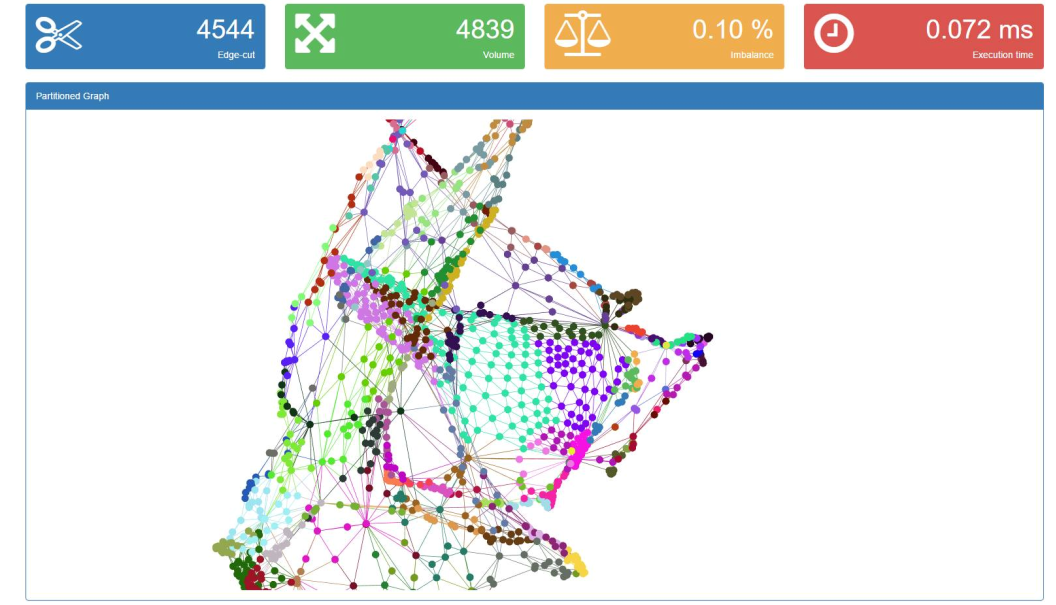
\includegraphics[width=0.8\textwidth]{ressources/graph}
\label{resultexample}
\caption{Result exemple}
\end{figure}

\paragraph{}
One can see from the screenshot available on figure \ref{resultexample}, nodes on the graph are painted into different color which indicates the partition. The edge-cut value, volume value, imbalance value is calculated and displayed as well as the execution time which is in order of second. 

\newpage
\appendix

\section{Meeting report : 11/01/15}

\subsection*{Details}
{\centering
\begin{tabular}{|c|c|c|}
    \hline
     Date & Attending & Report writer \\\hline
     \begin{tabular}{c}
     	11/01/2015\\
     	3:30pm - 4:00pm
     \end{tabular} & 
     \begin{tabular}{c}
     	Diaferia Quentin\\
     	Levasseur Thibaud\\ 
     	Pei Wang\\
     	Perez Bada Gonzalo
     \end{tabular} & 
     Diaferia Quentin \\\hline
\end{tabular}
\par}
\subsection*{Agenda}

\begin{itemize}
	\item Debriefing about the first week
	\item Tools
	\item Legal aspects
	\item Priorities
\end{itemize}

\subsection*{Debriefing about the first week}

\paragraph{}
Our goal is to realise a web graphic interface for Astral. It means that our users need to have an Astral account.

\paragraph{}
A prototype of the interface has been made using a bootstrap template and is available on Quentin's public web space : \url{http://public.cranfield.ac.uk/s242734/meshslicer/pages/index.html}

\paragraph{}
Thibaud has began to work on an algorithm to display a graph. It works, but it is extremely slow as the graph contains millions of vertices. It might be useless to display the whole graph, using a coarsened one should be enough to have a preview of the partitioned graph.

\section*{Tools}

\paragraph{}
We have set up a Trello and a Github repository to help us with the project management and the development. Fanny does not have her accounts yet, but will create them and learn to use those tools.

\paragraph{}
A technical issue about how to use SSH on a web application has been raised, but after a short research, we found that some PHP libraries exist and are easy to use.

\section*{Legal aspects}

\paragraph{}
Is it possible to "sell" an Astral account in addition of our web app to our customer ? We have to study the legal aspect. We are considering three different kinds of customers :
\begin{itemize}
	\item People having an Astral account
	\item People having their own HPC facility
	\item People not having any Astral account
\end{itemize}

\section*{Priorities}

\paragraph{}
We will visit the Cranfield IT department to ask whether it is possible to have an agreement with an external company to use Astral.

\paragraph{}
As soon as this question is answered, we will meet again to discuss the requirements and split the work.

\newpage
\section{Meeting report : 13/01/15}

\subsection*{Details}
{\centering
\begin{tabular}{|c|c|c|}
    \hline
     Date & Attending & Report writer \\\hline
     \begin{tabular}{c}
     	11/01/2015\\
     	11:30am - 12:10pm
     \end{tabular} & 
     \begin{tabular}{c}
     	Diaferia Quentin\\
     	Levasseur Thibaud\\ 
     	Pei Wang\\
     	Perez Bada Gonzalo
     \end{tabular} & 
     Thibaud Levasseur \\\hline
\end{tabular}
\par}
\subsection*{Agenda}
The following topics were discuss in this meeting :
\begin{itemize}
	\item Question to the IT department;
	\item Client definition;
	\item Work split.
\end{itemize}

\subsection*{Question to the IT department}
After the last meeting, the whole group went to the IT department to ask if there were any kind of agreement between private companies and Cranfield related to the use of the Grid or Astral.
\paragraph{} As a lot of licence are bought as educational, it is not legal to resell it to private entities. Thus the software we aim to create will not be sold as a SaaS to the end user.

\subsection*{Client definition}
As the IT department said, our software could not be set on a SaaS business model unless we buy our own computational infrastructure. 
\paragraph{}Thibaud raised the idea to actually sell the software to the owner of the computational resources and not to the end user. So, each entity willing to give to its user an easy interface to use instead of a command line terminal might be interested by our application.

\subsection*{Work split}
Short term objectives were define during this meeting, with piece of work splitting among the team.

\paragraph{Diaferia Quentin}
\begin{itemize}
	\item Organizes Git repository;
	\item Writes  the requirements of the upload and download of files;
	\item Commits his work on Github;
	\item Implement the Login on Astral
\end{itemize}

\paragraph{Levasseur Thibaud}
\begin{itemize}
	\item Writes  the requirements of the authentication;
	\item Commits his work on Github;
	\item Implement the Login on Astral
\end{itemize}

\paragraph{Pei Wang}
\begin{itemize}
	\item Register on Github and learn how to use it;
	\item Register on Trello and learn how to use it;
	\item Writes  the display requirements;
	\item Writes  the non functional requirements;

\end{itemize}

\paragraph{Perez Bada Gonzalo}
\begin{itemize}
	\item Writes  the requirements of the script use (Metis);
\end{itemize}


\newpage
\section{Meeting report 04/03/15}

\subsection*{Details}
{\centering
\begin{tabular}{|c|c|c|}
    \hline
     Date & Attending & Report writer \\\hline
     \begin{tabular}{c}
     	04/03/2015\\
     	10:30am - 10:45pm
     \end{tabular} & 
     \begin{tabular}{c}
     	Diaferia Quentin\\
     	Levasseur Thibaud\\ 
     	Pei Wang\\
     	Perez Bada Gonzalo
     \end{tabular} & 
     Thibaud Levasseur \\\hline
\end{tabular}
\par}
\subsection*{Agenda}
The following topics were discuss in this meeting :
\begin{itemize}
	\item What have been done;
	\item What is left to do.
	
\end{itemize}


\subsection*{What have been done}
\paragraph{Interface}
The interface is almost done : downloading a file has still some issues. The file stay on the server after copied from Astral. It is required to be deleted at some point.
\paragraph{Configuration file}
Creating the configuration file is now possible through the application.
\paragraph{C program}
The program is working on both mesh and graphs. It is now properly documented
\paragraph{Graph displayer}
The display works independently from the Interface. It reduces the size of the graph and color it properly. It needs to be integrated in the interface. Mesh file are not yet taken into account.

\subsection*{What is left to do}
The following point are still to be done :
\begin{itemize}
	\item Integrate the graph displayer;
	\item Create the link between the interface and the program;
	\item Fill up the landing page advertising;
	\item Adapt the graph displayer to meshes;
	\item Parse the output file;
	\item Test the program in order to find possible bugs.
\end{itemize}
 

\newpage
\section{Meeting report 09/03/15}

\subsection*{Details}
{\centering
\begin{tabular}{|c|c|c|}
    \hline
     Date & Attending & Report writer \\\hline
     \begin{tabular}{c}
     	04/03/2015\\
     	11:30am - 12pm
     \end{tabular} & 
     \begin{tabular}{c}
     	Diaferia Quentin\\
     	Levasseur Thibaud\\
     \end{tabular} & 
     Thibaud Levasseur \\\hline
\end{tabular}
\par}
\subsection*{Agenda}
The following topics were discuss in this meeting :
\begin{itemize}
	\item Debugging graphical interface;
	\item Improvement clue;
	\item Shooting demo video.
	
\end{itemize}


\subsection*{Debugging graphical interface}
Some bugs does still exists :
\begin{itemize}
	\item When partitioning a mesh, a radio button was displayed instead of the 'eye' button;
	\item 'Launch partitioning' was sometimes called two times
\end{itemize}
\subsection*{Improvement Clue}
The following idea were described for further improvement:
\begin{itemize}
	\item Display mesh as graph are;
	\item Enable the user to use paraMetis;
	\item Display to the user the setting chosen previously;
	\item Create a user guide on the web site;
	\item Add a countdown in the logout page.
\end{itemize} 
\subsection*{Shooting demo video}
As Astral is not always fast working, it has been decided to shoot a video in order to have a B plan if the demo is not working properly during the presentation of the 10/03/2016.
\newpage
\section{Meeting report 24/03/15}

\subsection*{Details}
{\centering
	\begin{tabular}{|c|c|c|}
		\hline
		Date & Attending & Report writer \\\hline
		\begin{tabular}{c}
			04/03/2015\\
			11:30am - 12pm
		\end{tabular} & 
		\begin{tabular}{c}
			Diaferia Quentin\\
			Levasseur Thibaud\\ 
			Pei Wang\\
			Perez Bada Gonzalo
		\end{tabular} & 
		Perez Bada Gonzalo \\\hline
	\end{tabular}
	\par}
\subsection*{Agenda}
The following topics were discuss in this meeting :
\begin{itemize}
	\item Final product delivery;
	\item Final report;
	\item Potential improvements;
	
\end{itemize}


\subsection*{Final product delivery}
Basic elements to deliver :
\begin{itemize}
	\item Working virtual machine with the working website installed on a localhost;
	\item Partitioning application code
	\item Web page source code
	\item Final report
\end{itemize}
\subsection*{Final report}
All the sections of the report were checked:
\begin{itemize}
	\item Technical report;
	\item Workload distribution;
	\item Project management and work tasks;
	\item Potential improvements;
	\item Appendixes, including sub-products and the meeting agendas.
\end{itemize} 
\subsection*{Potential improvements}
The team dedicated some extra time to define possible new features and functionality fixes for the application in future versions, and included a list in the report as a new section.
\newpage
\section{Trello}

\begin{figure}[h!]
\centering
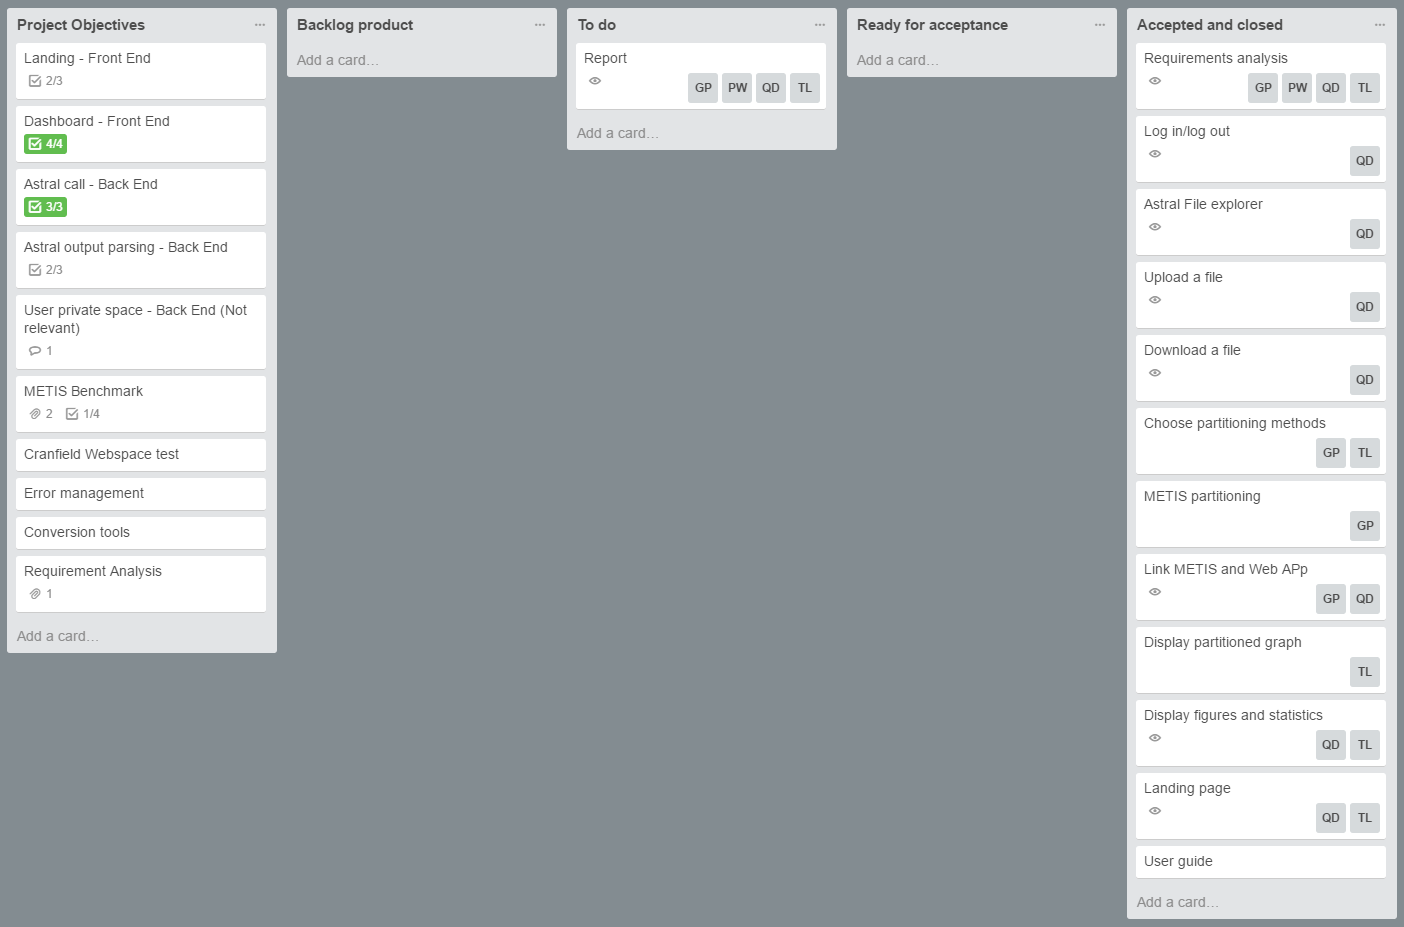
\includegraphics[width=1\textwidth]{ressources/trello}
\label{trello}
\caption{Trello, screenshot taken during the redaction of this report}
\end{figure}

\newpage

\section{Libraries}
\begin{itemize}
\item Bootstrap : http://getbootstrap.com/
\item JQuery : https://jquery.com/
\item JSDropzone : http://www.dropzonejs.com/
\item PHPseclib : http://phpseclib.sourceforge.net/
\item SigmaJS : http://sigmajs.org/
\end{itemize}


\end{document}
